\documentclass[10pt]{article}
\usepackage{../pplmanual}
%%% Commonly Needed packages
\usepackage{graphicx,color,calc}
\usepackage{fancyvrb}
\usepackage{makeidx}
\usepackage{alltt}
\usepackage{html}
\usepackage{hyphenat}
\usepackage{listings}
\usepackage{xspace} %<- creates problems with other hyperlink packages like "html"
\usepackage{hyperref}
\hypersetup{
    colorlinks,%
    citecolor=black,%
    filecolor=black,%
    linkcolor=black,%
    urlcolor=magenta
}


%%% Commands for uniform looks of C++, Charm++, and Projections
\newcommand{\CC}{C\hbox{++}\xspace}
\newcommand{\emCC}{C\hbox{\em++}\xspace}
\newcommand{\charmpp}{Charm++\xspace}
\newcommand{\charm}{Charm++\xspace}
\newcommand{\charmc}{\texttt{charmc}\xspace}
\newcommand{\projections}{\textrm{Projections}\xspace}
\newcommand{\converse}{Converse\xspace}
\newcommand{\ampi}{\textup{AMPI}\xspace}
\newcommand{\tempo}{\textsc{TeMPO}\xspace}
\newcommand{\irecv}{\textsl{iRecv}\xspace}
\newcommand{\sdag}{\textsl{Structured Dagger}\xspace}
\newcommand{\jade}{Jade\xspace}
\newcommand{\ci}{\emph{ci}\xspace}

%%% Commands to produce margin symbols
\newcommand{\new}{\marginpar{\fbox{\bf$\mathcal{NEW}$}}}
\newcommand{\important}{\marginpar{\fbox{\bf\Huge !}}}
\newcommand{\experimental}{\marginpar{\fbox{\bf\Huge $\beta$}}}

%%% Commands for manual elements
\newcommand{\zap}[1]{ }
\newcommand{\function}[1]{{\noindent{\textsf{#1}}\\}}
\newcommand{\cmd}[1]{{\noindent{\textsf{#1}}\\}}
\newcommand{\args}[1]{\hspace*{2em}{\texttt{#1}}\\}
\newcommand{\prototype}[1]{\vspace{0.2in}\index{#1}}
\newcommand{\param}[1]{{\texttt{#1}}}
\newcommand{\kw}[1]{{\nohyphens{\textsf{#1}}\index{#1}}}
\newcommand{\uw}[1]{#1}
\newcommand{\desc}[1]{\indent{#1}}
\newcommand{\note}[1]{(\textbf{Note:} #1)}
\newcommand{\term}[1]{{\bf #1}\index{#1}}

% Explicitly state that part numbering uses uppercase roman numerals
% This is just to keep latex2html from barfing and causing a filename
% collision between part II and chapter 2 etc. This will work as long
% as we don't have an appendix section 9 (which would be alphabetized
% to I (and again conflict with part 1).
\renewcommand{\thepart}{\Roman{part}}

\newcommand{\gitweb}[2]{http://charm.cs.illinois.edu/cgi-bin/gitweb2.cgi?p=charm.git;hb=HEAD;a=#1;f=#2}

\newcommand{\gitwebref}[3]{\href{\gitweb{#1}{#2/charm\%2B\%2B/#3}}{\tt #2/charm++/#3}}
\newcommand{\examplereffile}[1]{\gitwebref{blob}{examples}{#1}}
\newcommand{\examplerefdir}[1]{\gitwebref{tree}{examples}{#1}}
\newcommand{\testreffile}[1]{\gitwebref{blob}{tests}{#1}}
\newcommand{\testrefdir}[1]{\gitwebref{tree}{tests}{#1}}

\begin{htmlonly}
\renewcommand{\examplereffile}[1]{\texttt{\emph{examples/charm++/#1}}}
\renewcommand{\examplerefdir}[1]{\texttt{examples/charm++/#1}}
\renewcommand{\testreffile}[1]{\texttt{\emph{tests/charm++/#1}}}
\renewcommand{\testrefdir}[1]{\texttt{tests/charm++/#1}}
\end{htmlonly}
\makeindex


\title{BigSimulator (BigNetSim) for Extremely Large Parallel Machines}
\version{1.01}
	\credits{The Charm++ BigSim Emulator was developed by Arun Singla,
Neelam Saboo and Joshua Unger under the guidance of Prof. L. V. Kale. The new
Converse BigSim Emulator was completely rewritten by Gengbin Zheng. The
Converse BigSim Emulator is the only version under maintenance now. Charm++ and
Adaptive MPI (AMPI) were ported onto the BigSim Emulator by Gengbin Zheng. The
parallel performance simulator was developed by Gengbin Zheng and Gunavardhan
Kakulapati. A postmortem network simulator was developed by Terry Wilmarth,
Eric Bohm and Gengbin Zheng}

\begin{document}
\maketitle

\section{BigSim Network Simulator}
\label{bignetsim}

The BigSim Network Simulator is also known as Bigsimulator and lives
in the SVN repository https://charm.cs.uiuc.edu/svn/repos/BigNetSim.
The Network simulator is actually more of an Inter-connection network
simulator and hence more important in the context of large parallel
machines with interconnects.
The BigSim simulator  along with the network simulator is together
also known as BigNetSim.

Both the simulators run on top of the POSE framework, which is a Parallel
Discrete Event Simulation framework built on top of \charmpp{}.


\subsection{What does this software do?}
BigNetSim is an effort to simulate large current and future computer
systems to study the behavior of applications developed for those systems.
BigNetSim could be used to study
\begin{itemize}
\item  new types of interconnection topologies and routing algorithms
along with different types of switching architecture.
\item application performance on different machines. This uses the API
provided in Section \ref{bgapi} to run the application on some number
of processors on some machine and generate (dump) all events (entry
method executions or message send/recv).  BigNetSim is used to
model the machine that needs to be studied for this application and
these logs are then fed into this simulation, and it predicts the
performance of this application.
\end{itemize}

So, the two important uses are studying {\it interconnection networks} and
{\it performance prediction for applications}.

\charmpp{} can be installed either from the source code or using a precompiled
binary package. Building from the source code provides more flexibility, since one 
can choose the options as desired. However, a precompiled binary may be slightly
easier to get running.
 
\section{Downloading \charmpp{}}

\charmpp{} can be downloaded using one of the following methods:

\begin{itemize}
\item From \charmpp{} website -- The current stable version (source code and
binaries) can be downloaded from our website at {\em http://charm.cs.illinois.edu/software}.
\item From source archive -- The latest development version of \charmpp{} can be downloaded
from our source archive using {\em git clone http://charm.cs.illinois.edu/gerrit/charm}.
\end{itemize}

If you download the source code from the website, you will have to unpack it 
using a tool capable of extracting gzip'd tar files, such as tar (on Unix) 
or WinZIP (under Windows).  \charmpp{} will be extracted to a directory 
called ``charm''. 

\section{Installation}

A typical prototype command for building \charmpp{} from the source code is:
\vspace{5pt}\\
{\bf ./build $<$TARGET$>$ $<$TARGET ARCHITECTURE$>$ [OPTIONS]} where,

\begin{description}
\item [TARGET] is the framework one wants to build such as {\em charm++} or {\em
AMPI}.
\item [TARGET ARCHITECTURE] is the machine architecture one wants to build for
such as {\em net-linux-x86\_64}, {\em bluegenep} etc.
\item [OPTIONS] are additional options to the build process, e.g. {\em smp} is
used to build a shared memory version, {\em -j8} is given to build in parallel
etc.
\end {description}

In Table~\ref{tab:buildlist}, a list of build commands is provided for some of the commonly 
used systems. Note that, in general, options such as {\em smp},
\verb|--with-production|, compiler specifiers etc can be used with all targets.
It is advisable to build with \verb|--with-production| to obtain the best
performance.  If one desires to perform trace collection (for Projections),
\verb|--enable-tracing --enable-tracing-commthread| should also be passed to the
build command.

Details on all the available alternatives for each of the above mentioned
parameters can be found by invoking \verb|./build --help|. One can also go through the
build process in an interactive manner. Run \verb|./build|, and it will be followed by
a few queries to select appropiate choices for the build one wants to perform.


\begin{table}[ht]
\begin{tabular}{|p{6cm}|p{9cm}|}
\hline
Net with 32 bit Linux & \verb|./build charm++ net-linux --with-production -j8|
\\\hline
Multicore 64 bit Linux & \verb|./build charm++ multicore-linux64 --with-production -j8|
\\\hline
Net with 64 bit Linux & \verb|./build charm++ net-linux-x86_64 --with-production -j8|
\\\hline
Net with 64 bit Linux (intel compilers) & \verb|./build charm++ net-linux-x86_64 icc --with-production -j8|
\\\hline
Net with 64 bit Linux (shared memory) & \verb|./build charm++ net-linux-x86_64 smp --with-production -j8|
\\\hline
Net with 64 bit Linux (checkpoint restart based fault tolerance) & \verb|./build charm++ net-linux-x86_64 syncft --with-production -j8|
\\\hline
MPI with 64 bit Linux & \verb|./build charm++ mpi-linux-x86_64 --with-production -j8|
\\\hline
MPI with 64 bit Linux (shared memory) & \verb|./build charm++ mpi-linux-x86_64 smp --with-production -j8|
\\\hline
MPI with 64 bit Linux (mpicxx wrappers) & \verb|./build charm++ mpi-linux-x86_64 mpicxx --with-production -j8|
\\\hline
IBVERBS with 64 bit Linux & \verb|./build charm++ net-linux-x86_64 ibverbs --with-production -j8|
\\\hline
Net with 32 bit Windows & \verb|./build charm++ net-win32 --with-production -j8|
\\\hline
Net with 64 bit Windows & \verb|./build charm++ net-win64 --with-production -j8|
\\\hline
MPI with 64 bit Windows & \verb|./build charm++ mpi-win64 --with-production -j8|
\\\hline
Net with 64 bit Mac & \verb|./build charm++ net-darwin-x86_64 --with-production -j8|
\\\hline
Blue Gene/L & \verb|./build charm++ bluegenel xlc --with-production -j8|
\\\hline
Blue Gene/P & \verb|./build charm++ bluegenep xlc --with-production -j8|
\\\hline
Blue Gene/Q & \verb|./build charm++ pami-bluegeneq xlc --with-production -j8|
\\\hline
Blue Gene/Q & \verb|./build charm++ pamilrts-bluegeneq xlc --with-production -j8|
\\\hline
Cray XT3 & \verb|./build charm++ mpi-crayxt3 --with-production -j8|
\\\hline
Cray XT5 & \verb|./build charm++ mpi-crayxt --with-production -j8|
\\\hline
Cray XE6 & \verb|./build charm++ gemini_gni-crayxe --with-production -j8|
\\\hline
\end{tabular}
\caption{Build command for some common cases}
\label{tab:buildlist}
\end{table}

As mentioned earlier, one can also build \charmpp{} using the precompiled binary
in a manner similar to what is used for installing any common software.


The main directories in a \charmpp{} installation are:

\begin{description}
\item[\kw{charm/bin}]
Executables, such as charmc and charmrun,
used by \charmpp{}.

\item[\kw{charm/doc}]
Documentation for \charmpp{}, such as this
document.  Distributed as LaTeX source code; HTML and PDF versions
can be built or downloaded from our web site.

\item[\kw{charm/include}]
The \charmpp{} C++ and Fortran user include files (.h).

\item[\kw{charm/lib}]
The libraries (.a) that comprise \charmpp{}.

\item[\kw{charm/examples}]
Example \charmpp{} programs.

\item[\kw{charm/src}]
Source code for \charmpp{} itself.

\item[\kw{charm/tmp}]
Directory where \charmpp{} is built.

%\item[\kw{charm/tools}]
%Visualization tools for \charmpp{} programs.

\item[\kw{charm/tests}]
Test \charmpp{} programs used by autobuild.

\end{description}

\section{Security Issues}

On most computers, \charmpp{} programs are simple binaries, and they pose
no more security issues than any other program would.  The only exception
is the network version {\tt net-*}, which has the following issues. 

The network versions utilize many unix processes communicating with
each other via UDP.  Only a simple attempt is currently made to filter out
unauthorized packets.  Therefore, it is theoretically possible to
mount a security attack by sending UDP packets to an executing
\converse{} or \charmpp{} program's sockets.

The second security issue associated with networked programs is
associated with the fact that we, the \charmpp{} developers, need evidence
that our tools are being used.  (Such evidence is useful in convincing
funding agencies to continue to support our work.)  To this end, we
have inserted code in the network {\tt charmrun} program (described
later) to notify us that our software is being used.
This notification is a single {\tt UDP} packet sent by {\tt charmrun}
to {\tt charm.cs.illinois.edu}.  This data is put
to one use only: it is gathered into tables recording the internet
domains in which our software is being used, the number of individuals
at each internet domain, and the frequency with which it is used.

We recognize that some users may have objections to our notification
code.  Therefore, we have provided a second copy of the {\tt
charmrun} program with the notification code removed.  If you look
within the {\tt bin} directory, you will find these programs:

\begin{alltt}
    \$ cd charm/bin
    \$ ls charmrun*
    charmrun
    charmrun-notify
    charmrun-silent
\end{alltt}

The program {\tt charmrun.silent} has the notification code removed.  To
permanently deactivate notification, you may use the version without the
notification code:

\begin{alltt}
    \$ cd charm/bin
    \$ cp charmrun.silent charmrun
\end{alltt}

The only versions of \charmpp{} that ever notify us are 
the network versions.


\section{Reducing disk usage}

The charm directory contains a collection of example-programs and
test-programs.  These may be deleted with no other effects. You may 
also {\tt strip} all the binaries in {\tt charm/bin}.







\subsection{Using BigSimulator}

BigSimulator (BigNetSim) has 2 major modes.

\begin{itemize}
\item{ Trace based traffic simulation }
\item{Artificial traffic generation based simulation.
The mode of the simulator is governed by the $USE\_TRANSCEIVER$ parameter
in the netconfig file.  When set to 0, trace based simulation is used,
when set to 1, traffic generation is used.}
\end{itemize}

Trace based simulation.  This is used to study target application performance,
or detailed network performance when loaded by a specific application.

There are two command line parameters for traced based simulation.
\begin{alltt}
  ./charmrun +p2 ./bigsimulator arg1 arg2
\end{alltt}
\begin{alltt}
  arg1 = 0 => Latency only mode
         1 => Detailed contention model
  arg2 = N => starts execution at the time marked by skip point N (0 is start)
\end{alltt}

\subsubsection{Simple Latency Model}
To use the simple latency model, follow the setup procedure above, noting that
the files are located in the trunk/SimpleLatency directory. This will produce
the "bigsimulator" file.

The command line parameters used for this model are different.  The format is
as follows:

\begin{alltt}
  [charmrun +p#] bigsimulator -lat <latency> -bw <bandwidth>
               [-cpp <cost per packet> -psize <packet size>]
               [-winsize <window size>] [-skip] [-print\_params]
\end{alltt}

\begin{alltt}
  Latency (lat)         - type double; in microseconds
  Bandwidth (bw)        - type double; in GB/s
  Cost per packet (cpp) - type double; in microseconds
  Packet size (psize)   - type int; in bytes
  Window size (winsize) - type int; in log entries
\end{alltt}

The implemented equation is: $lat + (N/bw) + cpp \times (N/psize)$

Latency and bandwidth are required.  If cost per packet is given, then packet
size must be given, as well.  Otherwise, cost per packet defaults to 0.0.
Packet size, if given, must be a positive integer.

The -winsize flag allows the user to specify the size of the window (number of
log entries) used when reading in the bgTrace log files.  This is useful if the
log files are large.  If -winsize is not specified, the value defaults to 0,
which indicates that no windowing will be used (i.e., there will be one window
for each time line that is equal to the size of the time line).

As with the second parameter in the examples of part (a) of this section, the
-skip flag indicates that the simulation should skip forward to the time stamp
set during trace creation (see the BigSim tutorial talk from the 2008 Charm++
workshop).  If -skip is not included, then no skipping will occur.

The -print\_params flag is provided for debugging convenience.  When present,
the simple latency model parameters will be displayed during simulation
initilization.

\subsubsection{Artificial Traffic Models}
Artificial traffic generation based simulation is use to study the performance
of interconnects under standard network load schemes.

\begin{alltt}
  ./bigsimulator arg1 arg2 arg3 arg4 arg5 arg6
\end{alltt}
example
\begin{alltt}
  ./bigsimulator 1 2 3 100 2031 0.1
\end{alltt}

\begin{alltt}
  arg1 = 0 => Latency only mode
         1 => Detailed contention model
  arg2 = 1 => deterministic traffic
         2 => poisson traffic
  arg3 = 1 => KSHIFT
         2 => RING
         3 => BITTRANSPOSE
         4 => BITREVERSAL
         5 => BITCOMPLEMENT
         6 => UNIFORM\_DISTRIBUTION
  arg4 = number of packets
  arg5 = message size
  arg6 = load factor
\end{alltt}


\subsection{Which Interconnection networks are implemented?}
A large number of topologies and routing strategies are implemented in the
software. Here, we present a list of interconnection networks. For a complete
list of routing strategies, input/output VC selectors, refer to the
corresponding directories in the software.

\begin{itemize}
\item HyperCube
\item FatTree
\item DenseGraph
\item Three dimensional Mesh
\item K-ary-N-cube
\item K-ary-N-fly
\item K-ary-N-mesh
\item K-ary-N-tree
\item N-mesh
\item Hybrid of Fattree and Dense Graph
\item Hybrid of Fattree and HyperCube
\end{itemize}

\subsection{Build your own Interconnection network}
To build a new interconnection network, one has to create a new directory for
that interconnection network and then create the routing strategy, topology,
input virtual channel selection and output virtual channel selection strategies
for that network. If existing strategies could be used, then reuse them, but if
new ones are required, one has to write these new strategies in the
corresponding directories for routing, topology, etc.

The InitNetwork function must be provided in InitNetwork.C for this new
interconnection network. It builds up all the nodes and switches and NICs and
channels that form the network. Look at one of the existing interconnection
topologies for reference.



\subsection{BigNetSim Design and Internals}
\begin{figure}[!t]
\centering  
  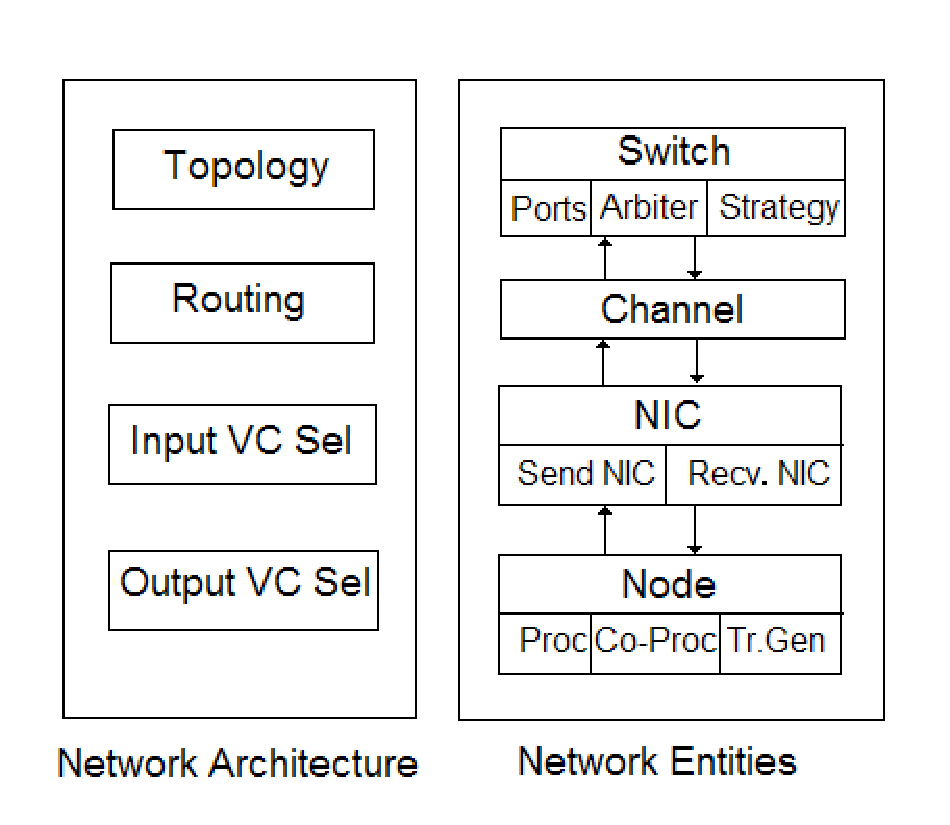
\includegraphics[width=3.2in]{figures/detailedsim_newer}
{\sffamily\bfseries\small \caption{BigNetSim conceptual model\label{fig:detailedsim_model}}}
\end{figure}

This section focuses on the interconnection network simulation.
The entities that form an interconnection network are:
\begin{itemize}
\item {\it switch:} A switch decides the routing on a packet. Switches could be
input buffered or output buffered. The former are implemented as individual posers
per port of each switch while the latter are implemented as a poser per switch.
In an {\it Input Buffered (IB)} switch, a packet in a switch is stored at the input 
port until its next route is decided and leaves the switch if it finds 
available space on the next switch in the route.
While in an {\it Output Buffered (OB)} switch, a packet in a switch decides beforehand 
on the next route to take and is buffered at the output port until space is
available on the next switch along the route.
Switches are modeled in much detail. Ports, buffers and
virtual channels at ports to avoid head-of-the-line blocking are
modeled.  Hardware collectives are implemented on the switch to
enable broadcasts, multicasts and other collective operations
efficiently. These are configurable and can be used if the system
being simulated supports them. We also support configurable
strategies for arbitration, input virtual channel selection and output
virtual channel selection. The configurability of the switch
provides a flexible design, satisfying the requirements of
a large number of networks.

\item {\it network card:} Network cards packetize and unpacketize messages.
A NIC is implemented as two posers. The sending and receiving entities in a
NIC are implemented as separate posers. A NIC is attached to each node.
\item {\it channel:} These are modeled as posers and connect a NIC to a switch
or a switch to another switch.
\item {\it compute node:} Each compute node connects to a network interface card.
A compute node simulates execution of entry methods on it. It is also attached
to a message traffic generator, which is used when only an interconnection
network is being simulated. This traffic generator can generate any message
pattern on each of the compute nodes.
The traffic generator can send
point-to-point messages, reductions, multicasts, broadcasts and other
collective traffic.  It supports k-shift, ring, bit-transpose,
bit-reversal, bit-complement and uniform random traffic.
These are based on common communication patterns found in
real applications. The frequency of message generation is determined
by a uniform or Poisson distribution.
\end{itemize}


\subsection{Topology, Routing and Virtual Channel Selection}
Topology, Routing strategies and input and output virtual channel selection
strategies need to be decided for any inter-connection network. Once we
have all of these in place we can simulate an inter-connection network.

\subsubsection{Topology}
For every architecture one wants to design, a topology file has to written
which defines a few basic functions for that particular topology.
These are:

\function{void getNeighbours(int nodeid, int numP);}
\index{getNeighbours}
\desc{This is called initially for every switch and this populates the
data structure {\it next} in a switch which contains the connectivity
of that switch. The switch specified by {\it switch} has {\it numP} ports.}

\function{int getNext(int portid, int nodeid, int numP)}
\index{getNext}
\desc{Returns the index of the switch/node that is connected to the
switch {\it nodeid}, at {\it portid}. The number of ports this node has is {\it numP}.}

\function{int getNextChannel(int portid, int nodeid, int numP)}
\index{getNextChannel}
\desc{Returns the index of the channel that is connected to the
switch {\it nodeid}, at {\it portid}. The number of ports this node has is {\it numP}.}

\function{int getStartPort(int nodeid, int numP, int dest)}
\index{getStartPort}
\desc{Return the index of the port that is connected to this compute node from a switch}

\function{int getStartVc()}
\index{getStartVc}
\desc{Returns the index of the first virtual channel (mostly 0).}

\function{int getStartSwitch(int nodeid)}
\index{getStartSwitch}
\desc{Returns the index of the node/switch that is connected to the first port}

\function{int getStartNode()}
\index{getStartNode}
\desc{Returns the index of the first node. Each poser has a separate index, 
irrespective of the type of the poser.}

\function{int getEndNode()}
\index{getEndNode}
\desc{Returns the index of the last node.}


\subsubsection{Routing}
Routing strategy needs to be specified for every interconnection network.
There is usually at least one routing strategy that needs to be defined
for every topology, Usually we have many more. The following functions need
to be defined for every routing strategy.

\function{int selectRoute(int current, int dest, int numP, Topology* top, Packet *p, map<int,int> \&bufsize, unsigned short *xsubi)}
\index{selectRoute}
\desc{Returns the portid that should be taken on switch {\it current} if the destination
is {\it dest}. The number of ports on a switch is {\it numP}. We also pass the pointer 
to the topology and to the Packet.}

\function{int selectRoute(int current, int dest, int numP, Topology* top, Packet *p, map<int,int> \&bufsize, map<int,int> \&portContention, unsigned short *xsubi)}
\index{selectRouteCont}
\desc{Returns the portid that should be taken on switch {\it current} if the destination
is {\it dest}. The number of ports on a switch is {\it numP}. We also pass the pointer 
to the topology and to the Packet. {\it Bufsize} is the state of the ports in
a switch, i.e. how many buffers on each port are full, while {\it portContention}
is used to give priority to certain ports, when more options are available.}

\function{int expectedTime(int src, int dest, POSE\_TimeType ovt, POSE\_TimeType origOvt, int length, int *numHops)}
\index{expectedTime}
\desc{Returns the expected time for a packet to travel from {\it src} to {\it dest},
when the number of hops it will need to travel is {\it numHops}.}

\function{int convertOutputToInputPort(int id, Packet *p, int numP, int *next)}
\index{convertOutputToInputPort}
\desc{Translate this output port to input port on the switch this port is
connected to.}


\subsubsection{Input Virtual Channel Selection}
For every switch, we need to know the mechanism it uses to choose input virtual channel.
There are a few different input virtual channel selection strategies, and a switch
can choose among them. Each should implement the following function.

\function{int selectInputVc(map<int,int> \&availBuffer, map<int,int> \&request, map<int,vector<Header> > \&inBuffer, int globalVc, int curSwitch)}
\index{selectInputVc}
\desc{Returns the input virtual channel to be used depending on the strategy and
the input parameters.}


\subsubsection{Output Virtual Channel Selection}
For every switch, we need to know the mechanism it uses to choose output virtual channel.
There are a few different output virtual channel selection strategies, and a switch
can choose among them. Each should implement the following function.

\function{int selectOutputVc(map<int,int> \&bufsize, Packet *p, int unused)}
\index{selectOutputVc}
\desc{Returns the output virtual channel to be used depending on the strategy and
the input parameters.}



\input{index}

\end{document}

